% Für Bindekorrektur als optionales Argument "BCORfaktormitmaßeinheit", dann
% sieht auch Option "twoside" vernünftig aus
% Näheres zu "scrartcl" bzw. "scrreprt" und "scrbook" siehe KOMA-Skript Doku
\documentclass[12pt,a4paper,titlepage,headinclude,bibtotoc]{scrartcl}


%---- Allgemeine Layout Einstellungen ------------------------------------------

% Für Kopf und Fußzeilen, siehe auch KOMA-Skript Doku
\usepackage[komastyle]{scrpage2}
\pagestyle{scrheadings}
\automark[section]{chapter}
\setheadsepline{0.5pt}[\color{black}]

%keine Einrückung
\parindent0pt

%Einstellungen für Figuren- und Tabellenbeschriftungen
\setkomafont{captionlabel}{\sffamily\bfseries}
\setcapindent{0em}


%---- Weitere Pakete -----------------------------------------------------------
% Die Pakete sind alle in der TeX Live Distribution enthalten. Wichtige Adressen
% www.ctan.org, www.dante.de

% Sprachunterstützung
\usepackage[ngerman]{babel}

% Benutzung von Umlauten direkt im Text
% entweder "latin1" oder "utf8"
\usepackage[utf8]{inputenc}

% Pakete mit Mathesymbolen und zur Beseitigung von Schwächen der Mathe-Umgebung
\usepackage{latexsym,exscale,amssymb,amsmath}

% Weitere Symbole
\usepackage[nointegrals]{wasysym}
\usepackage{eurosym}

% Anderes Literaturverzeichnisformat
%\usepackage[square,sort&compress]{natbib}

% Für Farbe
\usepackage{color}

% Zur Graphikausgabe
%Beipiel: \includegraphics[width=\textwidth]{grafik.png}
\usepackage{graphicx}

% Text umfließt Graphiken und Tabellen
% Beispiel:
% \begin{wrapfigure}[Zeilenanzahl]{"l" oder "r"}{breite}
%   \centering
%   \includegraphics[width=...]{grafik}
%   \caption{Beschriftung} 
%   \label{fig:grafik}
% \end{wrapfigure}
\usepackage{wrapfig}

% Mehrere Abbildungen nebeneinander
% Beispiel:
% \begin{figure}[htb]
%   \centering
%   \subfigure[Beschriftung 1\label{fig:label1}]
%   {\includegraphics[width=0.49\textwidth]{grafik1}}
%   \hfill
%   \subfigure[Beschriftung 2\label{fig:label2}]
%   {\includegraphics[width=0.49\textwidth]{grafik2}}
%   \caption{Beschriftung allgemein}
%   \label{fig:label-gesamt}
% \end{figure}
\usepackage{subfigure}

% Caption neben Abbildung
% Beispiel:
% \sidecaptionvpos{figure}{"c" oder "t" oder "b"}
% \begin{SCfigure}[rel. Breite (normalerweise = 1)][hbt]
%   \centering
%   \includegraphics[width=0.5\textwidth]{grafik.png}
%   \caption{Beschreibung}
%   \label{fig:}
% \end{SCfigure}
\usepackage{sidecap}

% Befehl für "Entspricht"-Zeichen
\newcommand{\corresponds}{\ensuremath{\mathrel{\widehat{=}}}}

%Für chemische Formeln (von www.dante.de)
%% Anpassung an LaTeX(2e) von Bernd Raichle
\makeatletter
\DeclareRobustCommand{\chemical}[1]{%
  {\(\m@th
   \edef\resetfontdimens{\noexpand\)%
       \fontdimen16\textfont2=\the\fontdimen16\textfont2
       \fontdimen17\textfont2=\the\fontdimen17\textfont2\relax}%
   \fontdimen16\textfont2=2.7pt \fontdimen17\textfont2=2.7pt
   \mathrm{#1}%
   \resetfontdimens}}
\makeatother

%Si Einheiten
\usepackage{siunitx}

%c++ Code einbinden
\usepackage{listings}
\lstset{numbers=left, numberstyle=\tiny, numbersep=5pt}

%errorFkt
\newcommand{\erf}{\ensuremath{\text{erf}}}

%Differential
\newcommand{\dif}{\ensuremath{\mathrm{d}}}

%Boxen,etc.
\usepackage{fancybox}
\usepackage{empheq}

%Fußnoten auf gleiche Seite
\interfootnotelinepenalty=1000


\begin{document}

\begin{titlepage}
\centering
\textsc{\Large Anfängerpraktikum der Fakultät für
  Physik,\\[1.5ex] Universität Göttingen}

\vspace*{4.2cm}

\rule{\textwidth}{1pt}\\[0.5cm]
{\huge \bfseries
  Spezifische Wärme der Luft und Gasthermometer\\[1.5ex]
  Protokoll:}\\[0.5cm]
\rule{\textwidth}{1pt}

\vspace*{2.0cm}

\begin{Large}
\begin{tabular}{ll}
Praktikant:
	&  Skrollan Detzler\\
 	&  Felix Kurtz\\
% 	&  Michael Lohmann\\
%	&  Kevin Lüdemann\\

  E-Mail: 
	&  skrollan.detzler@stud.uni-goettingen.de\\
	&  felix.kurtz@stud.uni-goettingen.de\\
%	& m.lohmann@stud.uni-goettingen.de\\
	
%	&  kevin.luedemann@stud.uni-goettingen.de\\

 Betreuer: & Martin Ochmann\\
 Versuchsdatum: & 02.06.2014\\
\end{tabular}
\end{Large}

\vspace*{0.8cm}

\begin{Large}
\fbox{
  \begin{minipage}[t][2.5cm][t]{6cm} 
    Testat:
  \end{minipage}
}
\end{Large}

\end{titlepage}

\tableofcontents

\newpage

\section{Einleitung}
\label{sec:einleitung}
Der erste Teil des Versuches dient der Bestimmung des absoluten Temperatur-Nullpunktes, eine der wichtigsten Naturkonstanten in der Thermodynamik.
Dies geschieht mithilfe eines Gasthermometers.\\
Im zweiten Teil bestimmt man die spezifische Wärme $c_V$ von Luft.
Diese gibt an, wie viel Energie pro Kilogramm benötigt wird, um sie um ein Kelvin zu erwärmen.

\section{Theorie}
\label{sec:theorie}
\subsection{Ideales Gas und Absoluter Temperaturnullpunkt}
Um Gase zu beschreiben benutzen wir hier das einfachste Modell, nämlich das des idealen Gases.
Dabei geht man von Punktteilchen aus.
Für mehratomige Gase wird diese Annahme immer ungenauer.\\
Die Abhängigkeiten zwischen Druck $p$, Volumen $V$ und Temperatur $T$ eines idealen Gases wird durch die folgende \textit{universelle Gasgleichung} \cite[S.261]{gerthsen} beschrieben.
\begin{align}
 p \cdot V = nRT
 \label{eq:uGasGl}
\end{align}
Dabei ist $R\approx 8.314 ~ \si{\joule \mol^{-1} \kelvin^{-1}}$ die universelle Gaskonstante und $n$ die Stoffmenge in Mol.
Hält man neben der Stoffmenge noch $V$ oder $p$ konstant, erhält man folgende Abhängigkeiten (Gesetze von Gay-Lussac \cite[S.261]{gerthsen}):
\begin{align}
	p(\vartheta)&=p_0 [1+\beta\vartheta] \quad, \quad V =\text{const.}
	\label{eq:p(T)}\\
	V(\vartheta)&=V_0 [1+\beta\vartheta] \quad, \quad p=\text{const.}	
\end{align}
Hierbei wird die Temperatur $\vartheta$ in Celsius gemessen, sodass $p_0$ der Druck und $V_0$ das Volumen bei $0\si{\celsius}$ ist.
Außerdem ist der Faktor $\beta=1/(273.15 \si{\celsius})$ der Umrechnung zwischen der Kelvin- und der Celsius-Skala geschuldet.\\
Aus obigen Gesetzmäßigkeiten kann der absolute Nullpunkt abgeleitet werden, der den Ursprung der absoluten Temperaturskala definiert, also $0~\si{\kelvin}=-273.15 \si{\celsius}=-1/\beta$.
Bei dieser Temperatur hätte jeder Stoff keine Ausdehnung.
Er ist jedoch experimentell nicht zu erreichen und kann per Extrapolation berechnet werden.

\subsection{Spezifische Wärme der Luft}
Die innere Energie $U$ eines Gases hängt proportional von seiner Temperatur ab \cite[S.257]{gerthsen}.
\begin{align}
	U=\frac{f}{2} n R T
\end{align}
Dabei ist $f$ die Anzahl der Freiheitsgrade des Gases.
Bei einem idealen Gas sind dies die 3 Raumrichtungen.
Mehratomige Gase können noch rotieren, etc.
So erhöht sich die Zahl der Freiheitsgrade entsprechend.\\

Der \textit{1.Hauptsatz} der Wärmelehre besagt nach \cite[S.262f.]{gerthsen}
\begin{align}
	\dif Q = \dif U+\dif W = \dif U+p\dif V \label{eq:1HS}
\end{align}

Aus der idealen Gasgleichung  folgt mit der Produktregel $R~\Delta T = p\Delta V+ V\Delta p$. Außerdem gilt für ideale Gase $U=c_VnT$ mit der spezifischen Wärme $c_V$ \cite[S.263]{gerthsen}.
Mit diesen Gleichungen sowie dem ersten Hauptsatz kann man nun die Anzahl der Freiheitsgrade bzw. die spezifische Wärme eines Gases berechnen:
\begin{align}
\frac{f}{2}=\frac{c_V}{R}
          &=\frac{\Delta U}{R~\Delta T}\notag\\
          &=\frac{\Delta Q-p\Delta V}{p\Delta V+V\Delta p} \label{eq:fhalbe}
\end{align}

Die in einem \textit{Kondensator} gespeicherte Energie lässt sich  durch Integration von $Q=CU$ nach $U$ berechnen \cite[S.329]{gerthsen}.
\begin{align}
	W=\int \limits_{0}^U Q ~\dif U'=\frac{1}{2}CU^2
	\label{eq:Kondensator}
\end{align}

\section{Durchführung}
\label{sec:durchfuehrung}
\subsection{Gasthermometer}
Bevor man mit dem eigentlichen Versuch beginnt, liest man am Barometer den Umgebungsdruck ab.
Dies wird später für die Auswertung benötigt.\\
Zuerst wird das Ventil des Druckmessgerätes geöffnet, um im Gaskolben Umgebungsdruck herzustellen.
Nun wird der Glaskolben durch Eiswasser auf etwa $0^\circ$ C herunter gekühlt.
Das Druckmessgerät sollte ungefähr 0 kPa anzeigen, da es nur Differenzen zum Umgebungsdruck angibt. Danach das Ventil schließen.\\
Nun wird die Heizplatte angeschaltet und damit das den Glaskolben umgebende Wasser auf bis zu $100^\circ$ C erhitzt.
Dabei misst man in $5^\circ$ C Schritten den Überdruck im Kolben.
Es ist also immer auf das Thermometer zu achten.
Außerdem muss das Wasser ständig umgerührt werden, um eine möglichst homogene Temperatur sicherzustellen.
Ferner sollte man bei hohen Temperaturen aufpassen, dass man sich nicht verbrüht.
Dann wird die Platte abgeschaltet, das Gefäß von dieser herunterbewegt und das Wasser mit Eis heruntergekühlt.
Dabei muss auf die Menge geachtet werden, da man auch beim Abkühlen den Druck in Abhängigkeit von der Temperatur messen soll.
Deshalb ist auch das Umrühren unerlässlich.
Des weiteren muss dafür gesorgt werden, dass das überlaufende Wasser aufgefangen wird. 
\begin{figure}[!h]
 \centering
 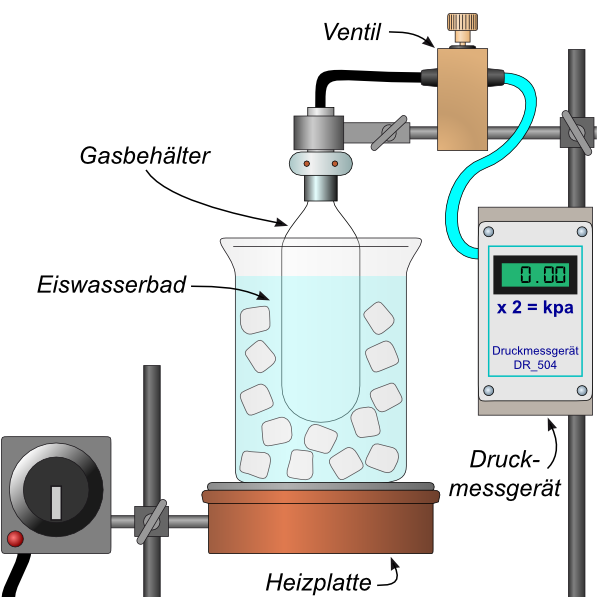
\includegraphics[scale=0.7]{GasthermometerSkizze.jpg}
 \caption{Skizze des Gasthermometers \cite{lp}}
 \label{fig:GTSkizze}
\end{figure}

\subsection{Spezifische Wärme der Luft}
\begin{figure}[!htb]
 \centering
 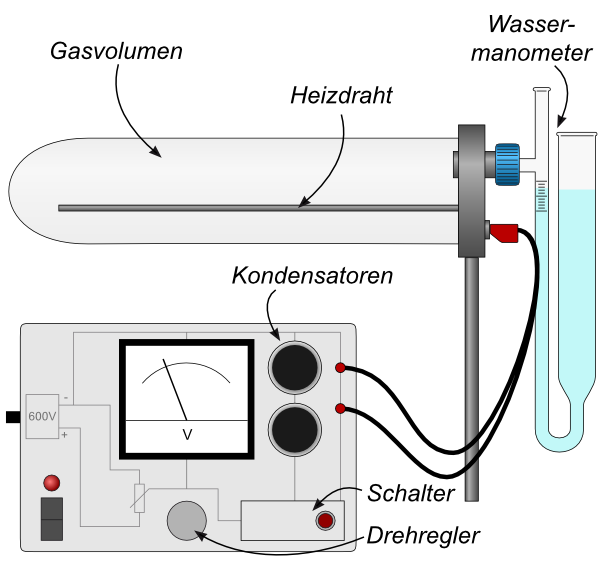
\includegraphics[scale=0.7]{SpezWaermeSkizze.jpg}
 \caption{schematischer Aufbau, um die spezifische Wärme von Luft zu messen \cite{lp}}
 \label{fig:SWLSkizze}
\end{figure}
Zuerst wird der Kondensator mit einer voreingestellten Spannung zwischen 100V und 500V geladen.
Diesen entlädt man daraufhin über den Heizdraht, während man parallel den Maximalausschlag des Manometers abliest.
Dieser Vorgang wird für mehrere Spannungen je dreimal wiederholt.
Zwischen den Messungen wird der Zylinder belüftet.
Zuletzt sollte das Ventil geöffnet zurückgelassen werden.\\
Ferner wird das Volumen des Zylinders gemessen.

%Auswertung und Diskussion von Michael&Kevin
\section{Auswertung}
\label{sec:auswertung}

\subsection{Gasthermometer}
Die Abbildungen \ref{fig:gas1} und \ref{fig:gas2} zeigen den Druck $p$ im Kolben in Abhängigkeit von der Temperatur - separat für Erwärmen und Abkühlen.
Da das Druckmessgerät nur Überdruck misst, muss der Umgebungsdruck addiert werden.
Außerdem steht auf dem Gerät, dass der angezeigte Wert verdoppelt werden muss, um den Überdruck in kPa zu erhalten.\\


Die Gleichung \eqref{eq:p(T)} besagt, dass ein linearer Zusammenhang  zwischen den beiden aufgetragenen Größen besteht:
$p(\vartheta)=m\vartheta+b$.
Der y-Achsenabschnitt $b$ ist der Umgebungsdruck $p_0$, die Steigung $m$ der Geraden das Produkt $p_0\beta$.
Für den Absoluten Nullpunkt $\vartheta_0$ ergibt sich also diese Formel und der zugehörige Fehler aus der Fehlerfortpflanzung
\begin{align}
	\vartheta_0&=-1/\beta=-\frac{b}{m}
	\label{eq:gas}\\
	\sigma_{\vartheta_0}&=\sqrt{\sigma_\text{b}^2\left(\frac{-1}{\text{m}}\right)^2+\sigma_\text{m}^2\left(\frac{\text{b}}{\text{m}^2}\right)^2}
	\label{eq:fegas}
\end{align}
 
\subsubsection{Erwärmen}
\label{sec:gas1}
\begin{figure}[!h]
\centering
% GNUPLOT: LaTeX picture with Postscript
\begingroup
  \makeatletter
  \providecommand\color[2][]{%
    \GenericError{(gnuplot) \space\space\space\@spaces}{%
      Package color not loaded in conjunction with
      terminal option `colourtext'%
    }{See the gnuplot documentation for explanation.%
    }{Either use 'blacktext' in gnuplot or load the package
      color.sty in LaTeX.}%
    \renewcommand\color[2][]{}%
  }%
  \providecommand\includegraphics[2][]{%
    \GenericError{(gnuplot) \space\space\space\@spaces}{%
      Package graphicx or graphics not loaded%
    }{See the gnuplot documentation for explanation.%
    }{The gnuplot epslatex terminal needs graphicx.sty or graphics.sty.}%
    \renewcommand\includegraphics[2][]{}%
  }%
  \providecommand\rotatebox[2]{#2}%
  \@ifundefined{ifGPcolor}{%
    \newif\ifGPcolor
    \GPcolortrue
  }{}%
  \@ifundefined{ifGPblacktext}{%
    \newif\ifGPblacktext
    \GPblacktexttrue
  }{}%
  % define a \g@addto@macro without @ in the name:
  \let\gplgaddtomacro\g@addto@macro
  % define empty templates for all commands taking text:
  \gdef\gplbacktext{}%
  \gdef\gplfronttext{}%
  \makeatother
  \ifGPblacktext
    % no textcolor at all
    \def\colorrgb#1{}%
    \def\colorgray#1{}%
  \else
    % gray or color?
    \ifGPcolor
      \def\colorrgb#1{\color[rgb]{#1}}%
      \def\colorgray#1{\color[gray]{#1}}%
      \expandafter\def\csname LTw\endcsname{\color{white}}%
      \expandafter\def\csname LTb\endcsname{\color{black}}%
      \expandafter\def\csname LTa\endcsname{\color{black}}%
      \expandafter\def\csname LT0\endcsname{\color[rgb]{1,0,0}}%
      \expandafter\def\csname LT1\endcsname{\color[rgb]{0,1,0}}%
      \expandafter\def\csname LT2\endcsname{\color[rgb]{0,0,1}}%
      \expandafter\def\csname LT3\endcsname{\color[rgb]{1,0,1}}%
      \expandafter\def\csname LT4\endcsname{\color[rgb]{0,1,1}}%
      \expandafter\def\csname LT5\endcsname{\color[rgb]{1,1,0}}%
      \expandafter\def\csname LT6\endcsname{\color[rgb]{0,0,0}}%
      \expandafter\def\csname LT7\endcsname{\color[rgb]{1,0.3,0}}%
      \expandafter\def\csname LT8\endcsname{\color[rgb]{0.5,0.5,0.5}}%
    \else
      % gray
      \def\colorrgb#1{\color{black}}%
      \def\colorgray#1{\color[gray]{#1}}%
      \expandafter\def\csname LTw\endcsname{\color{white}}%
      \expandafter\def\csname LTb\endcsname{\color{black}}%
      \expandafter\def\csname LTa\endcsname{\color{black}}%
      \expandafter\def\csname LT0\endcsname{\color{black}}%
      \expandafter\def\csname LT1\endcsname{\color{black}}%
      \expandafter\def\csname LT2\endcsname{\color{black}}%
      \expandafter\def\csname LT3\endcsname{\color{black}}%
      \expandafter\def\csname LT4\endcsname{\color{black}}%
      \expandafter\def\csname LT5\endcsname{\color{black}}%
      \expandafter\def\csname LT6\endcsname{\color{black}}%
      \expandafter\def\csname LT7\endcsname{\color{black}}%
      \expandafter\def\csname LT8\endcsname{\color{black}}%
    \fi
  \fi
  \setlength{\unitlength}{0.0500bp}%
  \begin{picture}(7200.00,5040.00)%
    \gplgaddtomacro\gplbacktext{%
      \csname LTb\endcsname%
      \put(1386,704){\makebox(0,0)[r]{\strut{} 1000}}%
      \put(1386,1213){\makebox(0,0)[r]{\strut{} 1050}}%
      \put(1386,1722){\makebox(0,0)[r]{\strut{} 1100}}%
      \put(1386,2231){\makebox(0,0)[r]{\strut{} 1150}}%
      \put(1386,2740){\makebox(0,0)[r]{\strut{} 1200}}%
      \put(1386,3249){\makebox(0,0)[r]{\strut{} 1250}}%
      \put(1386,3758){\makebox(0,0)[r]{\strut{} 1300}}%
      \put(1386,4267){\makebox(0,0)[r]{\strut{} 1350}}%
      \put(1386,4776){\makebox(0,0)[r]{\strut{} 1400}}%
      \put(1518,484){\makebox(0,0){\strut{} 0}}%
      \put(2062,484){\makebox(0,0){\strut{} 10}}%
      \put(2606,484){\makebox(0,0){\strut{} 20}}%
      \put(3150,484){\makebox(0,0){\strut{} 30}}%
      \put(3694,484){\makebox(0,0){\strut{} 40}}%
      \put(4238,484){\makebox(0,0){\strut{} 50}}%
      \put(4782,484){\makebox(0,0){\strut{} 60}}%
      \put(5326,484){\makebox(0,0){\strut{} 70}}%
      \put(5870,484){\makebox(0,0){\strut{} 80}}%
      \put(6414,484){\makebox(0,0){\strut{} 90}}%
      \put(6958,484){\makebox(0,0){\strut{} 100}}%
      \put(484,2740){\rotatebox{90}{\makebox(0,0){\strut{}Druck [hPa]}}}%
      \put(4238,154){\makebox(0,0){\strut{}Temperatur [$\si{\celsius}$]}}%
    }%
    \gplgaddtomacro\gplfronttext{%
      \csname LTb\endcsname%
      \put(5971,4603){\makebox(0,0)[r]{\strut{}Messwerte}}%
      \csname LTb\endcsname%
      \put(5971,4383){\makebox(0,0)[r]{\strut{}lineare Regression}}%
    }%
    \gplbacktext
    \put(0,0){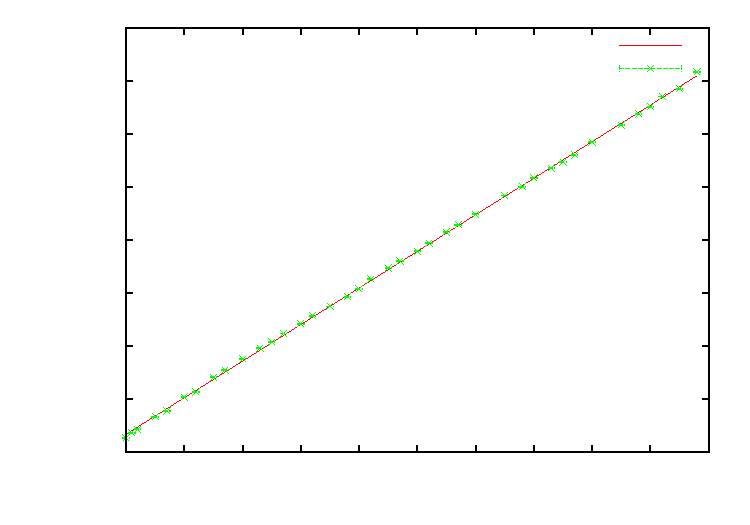
\includegraphics{gas1p}}%
    \gplfronttext
  \end{picture}%
\endgroup

\caption{Erwärmen: Druck als Funktion der Temperatur}
\label{fig:gas1}
\end{figure}
Die lineare Regression dieser Daten ergibt diese Werte für $m$ und $b$:
\begin{align*}
	\text{m} &= (345.1\pm0.9)\si{\pascal/\celsius}\\
	\text{b} &= (101640\pm50)\si{\pascal}\\
\end{align*}
Setzt man diese Werte in die obigen Formeln zur Bestimmung des absoluten Nullpunkts \eqref{eq:gas} und \eqref{eq:fegas} ein, ergibt sich:
$$\shadowbox{$\vartheta_0=(-294.5\pm0.8)\si{\celsius}$}$$

\subsubsection{Abkühlen}
\label{sec:gas2}
\begin{figure}[!h]
\centering
% GNUPLOT: LaTeX picture with Postscript
\begingroup
  \makeatletter
  \providecommand\color[2][]{%
    \GenericError{(gnuplot) \space\space\space\@spaces}{%
      Package color not loaded in conjunction with
      terminal option `colourtext'%
    }{See the gnuplot documentation for explanation.%
    }{Either use 'blacktext' in gnuplot or load the package
      color.sty in LaTeX.}%
    \renewcommand\color[2][]{}%
  }%
  \providecommand\includegraphics[2][]{%
    \GenericError{(gnuplot) \space\space\space\@spaces}{%
      Package graphicx or graphics not loaded%
    }{See the gnuplot documentation for explanation.%
    }{The gnuplot epslatex terminal needs graphicx.sty or graphics.sty.}%
    \renewcommand\includegraphics[2][]{}%
  }%
  \providecommand\rotatebox[2]{#2}%
  \@ifundefined{ifGPcolor}{%
    \newif\ifGPcolor
    \GPcolortrue
  }{}%
  \@ifundefined{ifGPblacktext}{%
    \newif\ifGPblacktext
    \GPblacktexttrue
  }{}%
  % define a \g@addto@macro without @ in the name:
  \let\gplgaddtomacro\g@addto@macro
  % define empty templates for all commands taking text:
  \gdef\gplbacktext{}%
  \gdef\gplfronttext{}%
  \makeatother
  \ifGPblacktext
    % no textcolor at all
    \def\colorrgb#1{}%
    \def\colorgray#1{}%
  \else
    % gray or color?
    \ifGPcolor
      \def\colorrgb#1{\color[rgb]{#1}}%
      \def\colorgray#1{\color[gray]{#1}}%
      \expandafter\def\csname LTw\endcsname{\color{white}}%
      \expandafter\def\csname LTb\endcsname{\color{black}}%
      \expandafter\def\csname LTa\endcsname{\color{black}}%
      \expandafter\def\csname LT0\endcsname{\color[rgb]{1,0,0}}%
      \expandafter\def\csname LT1\endcsname{\color[rgb]{0,1,0}}%
      \expandafter\def\csname LT2\endcsname{\color[rgb]{0,0,1}}%
      \expandafter\def\csname LT3\endcsname{\color[rgb]{1,0,1}}%
      \expandafter\def\csname LT4\endcsname{\color[rgb]{0,1,1}}%
      \expandafter\def\csname LT5\endcsname{\color[rgb]{1,1,0}}%
      \expandafter\def\csname LT6\endcsname{\color[rgb]{0,0,0}}%
      \expandafter\def\csname LT7\endcsname{\color[rgb]{1,0.3,0}}%
      \expandafter\def\csname LT8\endcsname{\color[rgb]{0.5,0.5,0.5}}%
    \else
      % gray
      \def\colorrgb#1{\color{black}}%
      \def\colorgray#1{\color[gray]{#1}}%
      \expandafter\def\csname LTw\endcsname{\color{white}}%
      \expandafter\def\csname LTb\endcsname{\color{black}}%
      \expandafter\def\csname LTa\endcsname{\color{black}}%
      \expandafter\def\csname LT0\endcsname{\color{black}}%
      \expandafter\def\csname LT1\endcsname{\color{black}}%
      \expandafter\def\csname LT2\endcsname{\color{black}}%
      \expandafter\def\csname LT3\endcsname{\color{black}}%
      \expandafter\def\csname LT4\endcsname{\color{black}}%
      \expandafter\def\csname LT5\endcsname{\color{black}}%
      \expandafter\def\csname LT6\endcsname{\color{black}}%
      \expandafter\def\csname LT7\endcsname{\color{black}}%
      \expandafter\def\csname LT8\endcsname{\color{black}}%
    \fi
  \fi
  \setlength{\unitlength}{0.0500bp}%
  \begin{picture}(7200.00,5040.00)%
    \gplgaddtomacro\gplbacktext{%
      \csname LTb\endcsname%
      \put(1386,704){\makebox(0,0)[r]{\strut{} 1000}}%
      \put(1386,1286){\makebox(0,0)[r]{\strut{} 1050}}%
      \put(1386,1867){\makebox(0,0)[r]{\strut{} 1100}}%
      \put(1386,2449){\makebox(0,0)[r]{\strut{} 1150}}%
      \put(1386,3031){\makebox(0,0)[r]{\strut{} 1200}}%
      \put(1386,3613){\makebox(0,0)[r]{\strut{} 1250}}%
      \put(1386,4194){\makebox(0,0)[r]{\strut{} 1300}}%
      \put(1386,4776){\makebox(0,0)[r]{\strut{} 1350}}%
      \put(1518,484){\makebox(0,0){\strut{} 0}}%
      \put(2062,484){\makebox(0,0){\strut{} 10}}%
      \put(2606,484){\makebox(0,0){\strut{} 20}}%
      \put(3150,484){\makebox(0,0){\strut{} 30}}%
      \put(3694,484){\makebox(0,0){\strut{} 40}}%
      \put(4238,484){\makebox(0,0){\strut{} 50}}%
      \put(4782,484){\makebox(0,0){\strut{} 60}}%
      \put(5326,484){\makebox(0,0){\strut{} 70}}%
      \put(5870,484){\makebox(0,0){\strut{} 80}}%
      \put(6414,484){\makebox(0,0){\strut{} 90}}%
      \put(6958,484){\makebox(0,0){\strut{} 100}}%
      \put(484,2740){\rotatebox{90}{\makebox(0,0){\strut{}Druck [hPa]}}}%
      \put(4238,154){\makebox(0,0){\strut{}Temperatur [$\si{\celsius}$]}}%
    }%
    \gplgaddtomacro\gplfronttext{%
      \csname LTb\endcsname%
      \put(5971,4603){\makebox(0,0)[r]{\strut{}Messwerte}}%
      \csname LTb\endcsname%
      \put(5971,4383){\makebox(0,0)[r]{\strut{}lineare Regression}}%
    }%
    \gplbacktext
    \put(0,0){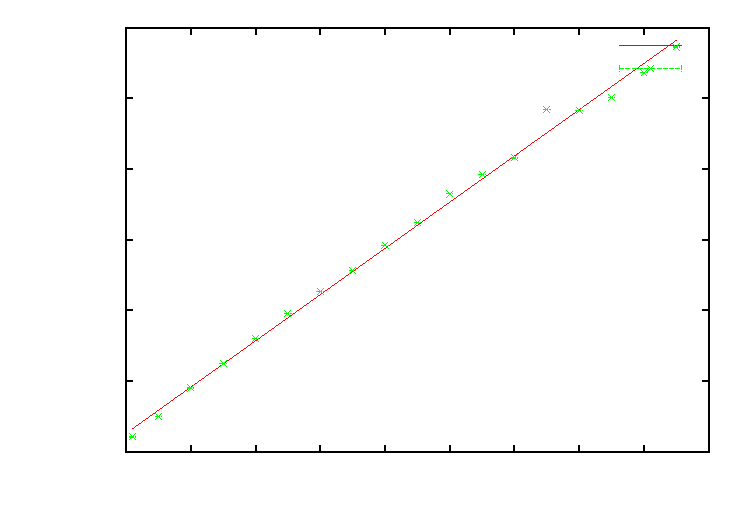
\includegraphics{gas2p}}%
    \gplfronttext
  \end{picture}%
\endgroup

\caption{Abkühlen: Druck als Funktion der Temperatur}
\label{fig:gas2}
\end{figure}
Aus der linearen Regression ergibt sich:
\begin{align}
	\text{m} &= (343\pm3)\si{\pascal/\celsius}\\
	\text{b} &= (101700\pm200)\si{\pascal}
\end{align}
Der daraus - wie zuvor - berechnete Nullpunkt liegt bei
$$\shadowbox{$\vartheta_0=(-297\pm3)\si{\celsius}$}$$

\subsubsection{Mittelwert}
Aus Erwärmen und Abkühlen kann jetzt der gewichteter Mittelwert gebildet werden.
Es ergibt sich:
$$\shadowbox{$\overline{\vartheta_0}=(-294.7\pm0.8)\si{\celsius}$}$$
Dies ist eine Abweichung von 8\% zum Literaturwert von $\vartheta_0=-273.15\si{\celsius}$.

\subsection{Spezifische Wärme von Luft}
\subsubsection{Freiheitsgrade der Luft}
Zum Berechnen der spezifischen Wärme von Luft $c_v$ bzw. der Freiheitsgrade des Gases, haben wir nach jeder Entladung der Kondensatoren die Steighöhe des Manometers notiert.
Diese muss jetzt in einen Druck umgerechnet werden.
Hierfür gilt die Formel $\Delta \rho = \rho_\text{Wasser} \cdot g \cdot h\left(1+\frac{r_1^2}{r_2^2}\right)$.
Die Werte für $r_1=2.0$mm und $r_2=9,2$mm sind aus der Praktikumsanleitung \cite[S. 73]{prakti}.
Die zugeführte Energie lässt sich durch die Formel \ref{eq:fhalbe} aus der Theorie berechnen.
Die Kapazität berechnet sich in unserem Fall aus zwei parallel geschalteten Kondensatoren mit einer Kapizät von je $10\mu$F, wieder aus der Praktikumsanleitung.
Die Graphik \ref{fig:druckwarm} zeigt die Druckänderung von Luft gegen die Kondensatorenergie aufgetragen.
\begin{figure}[!h]
\centering
% GNUPLOT: LaTeX picture with Postscript
\begingroup
  \makeatletter
  \providecommand\color[2][]{%
    \GenericError{(gnuplot) \space\space\space\@spaces}{%
      Package color not loaded in conjunction with
      terminal option `colourtext'%
    }{See the gnuplot documentation for explanation.%
    }{Either use 'blacktext' in gnuplot or load the package
      color.sty in LaTeX.}%
    \renewcommand\color[2][]{}%
  }%
  \providecommand\includegraphics[2][]{%
    \GenericError{(gnuplot) \space\space\space\@spaces}{%
      Package graphicx or graphics not loaded%
    }{See the gnuplot documentation for explanation.%
    }{The gnuplot epslatex terminal needs graphicx.sty or graphics.sty.}%
    \renewcommand\includegraphics[2][]{}%
  }%
  \providecommand\rotatebox[2]{#2}%
  \@ifundefined{ifGPcolor}{%
    \newif\ifGPcolor
    \GPcolortrue
  }{}%
  \@ifundefined{ifGPblacktext}{%
    \newif\ifGPblacktext
    \GPblacktexttrue
  }{}%
  % define a \g@addto@macro without @ in the name:
  \let\gplgaddtomacro\g@addto@macro
  % define empty templates for all commands taking text:
  \gdef\gplbacktext{}%
  \gdef\gplfronttext{}%
  \makeatother
  \ifGPblacktext
    % no textcolor at all
    \def\colorrgb#1{}%
    \def\colorgray#1{}%
  \else
    % gray or color?
    \ifGPcolor
      \def\colorrgb#1{\color[rgb]{#1}}%
      \def\colorgray#1{\color[gray]{#1}}%
      \expandafter\def\csname LTw\endcsname{\color{white}}%
      \expandafter\def\csname LTb\endcsname{\color{black}}%
      \expandafter\def\csname LTa\endcsname{\color{black}}%
      \expandafter\def\csname LT0\endcsname{\color[rgb]{1,0,0}}%
      \expandafter\def\csname LT1\endcsname{\color[rgb]{0,1,0}}%
      \expandafter\def\csname LT2\endcsname{\color[rgb]{0,0,1}}%
      \expandafter\def\csname LT3\endcsname{\color[rgb]{1,0,1}}%
      \expandafter\def\csname LT4\endcsname{\color[rgb]{0,1,1}}%
      \expandafter\def\csname LT5\endcsname{\color[rgb]{1,1,0}}%
      \expandafter\def\csname LT6\endcsname{\color[rgb]{0,0,0}}%
      \expandafter\def\csname LT7\endcsname{\color[rgb]{1,0.3,0}}%
      \expandafter\def\csname LT8\endcsname{\color[rgb]{0.5,0.5,0.5}}%
    \else
      % gray
      \def\colorrgb#1{\color{black}}%
      \def\colorgray#1{\color[gray]{#1}}%
      \expandafter\def\csname LTw\endcsname{\color{white}}%
      \expandafter\def\csname LTb\endcsname{\color{black}}%
      \expandafter\def\csname LTa\endcsname{\color{black}}%
      \expandafter\def\csname LT0\endcsname{\color{black}}%
      \expandafter\def\csname LT1\endcsname{\color{black}}%
      \expandafter\def\csname LT2\endcsname{\color{black}}%
      \expandafter\def\csname LT3\endcsname{\color{black}}%
      \expandafter\def\csname LT4\endcsname{\color{black}}%
      \expandafter\def\csname LT5\endcsname{\color{black}}%
      \expandafter\def\csname LT6\endcsname{\color{black}}%
      \expandafter\def\csname LT7\endcsname{\color{black}}%
      \expandafter\def\csname LT8\endcsname{\color{black}}%
    \fi
  \fi
  \setlength{\unitlength}{0.0500bp}%
  \begin{picture}(7200.00,5040.00)%
    \gplgaddtomacro\gplbacktext{%
      \csname LTb\endcsname%
      \put(1254,704){\makebox(0,0)[r]{\strut{} 0}}%
      \put(1254,1383){\makebox(0,0)[r]{\strut{} 50}}%
      \put(1254,2061){\makebox(0,0)[r]{\strut{} 100}}%
      \put(1254,2740){\makebox(0,0)[r]{\strut{} 150}}%
      \put(1254,3419){\makebox(0,0)[r]{\strut{} 200}}%
      \put(1254,4097){\makebox(0,0)[r]{\strut{} 250}}%
      \put(1254,4776){\makebox(0,0)[r]{\strut{} 300}}%
      \put(1386,484){\makebox(0,0){\strut{} 0}}%
      \put(2315,484){\makebox(0,0){\strut{} 0.5}}%
      \put(3243,484){\makebox(0,0){\strut{} 1}}%
      \put(4172,484){\makebox(0,0){\strut{} 1.5}}%
      \put(5101,484){\makebox(0,0){\strut{} 2}}%
      \put(6029,484){\makebox(0,0){\strut{} 2.5}}%
      \put(6958,484){\makebox(0,0){\strut{} 3}}%
      \put(484,2740){\rotatebox{90}{\makebox(0,0){\strut{}$\Delta p$ [Pa]}}}%
      \put(4172,154){\makebox(0,0){\strut{}$\Delta Q$ [J]}}%
    }%
    \gplgaddtomacro\gplfronttext{%
      \csname LTb\endcsname%
      \put(3894,4603){\makebox(0,0)[r]{\strut{}Messwerte}}%
      \csname LTb\endcsname%
      \put(3894,4383){\makebox(0,0)[r]{\strut{}Lineare Regression}}%
    }%
    \gplbacktext
    \put(0,0){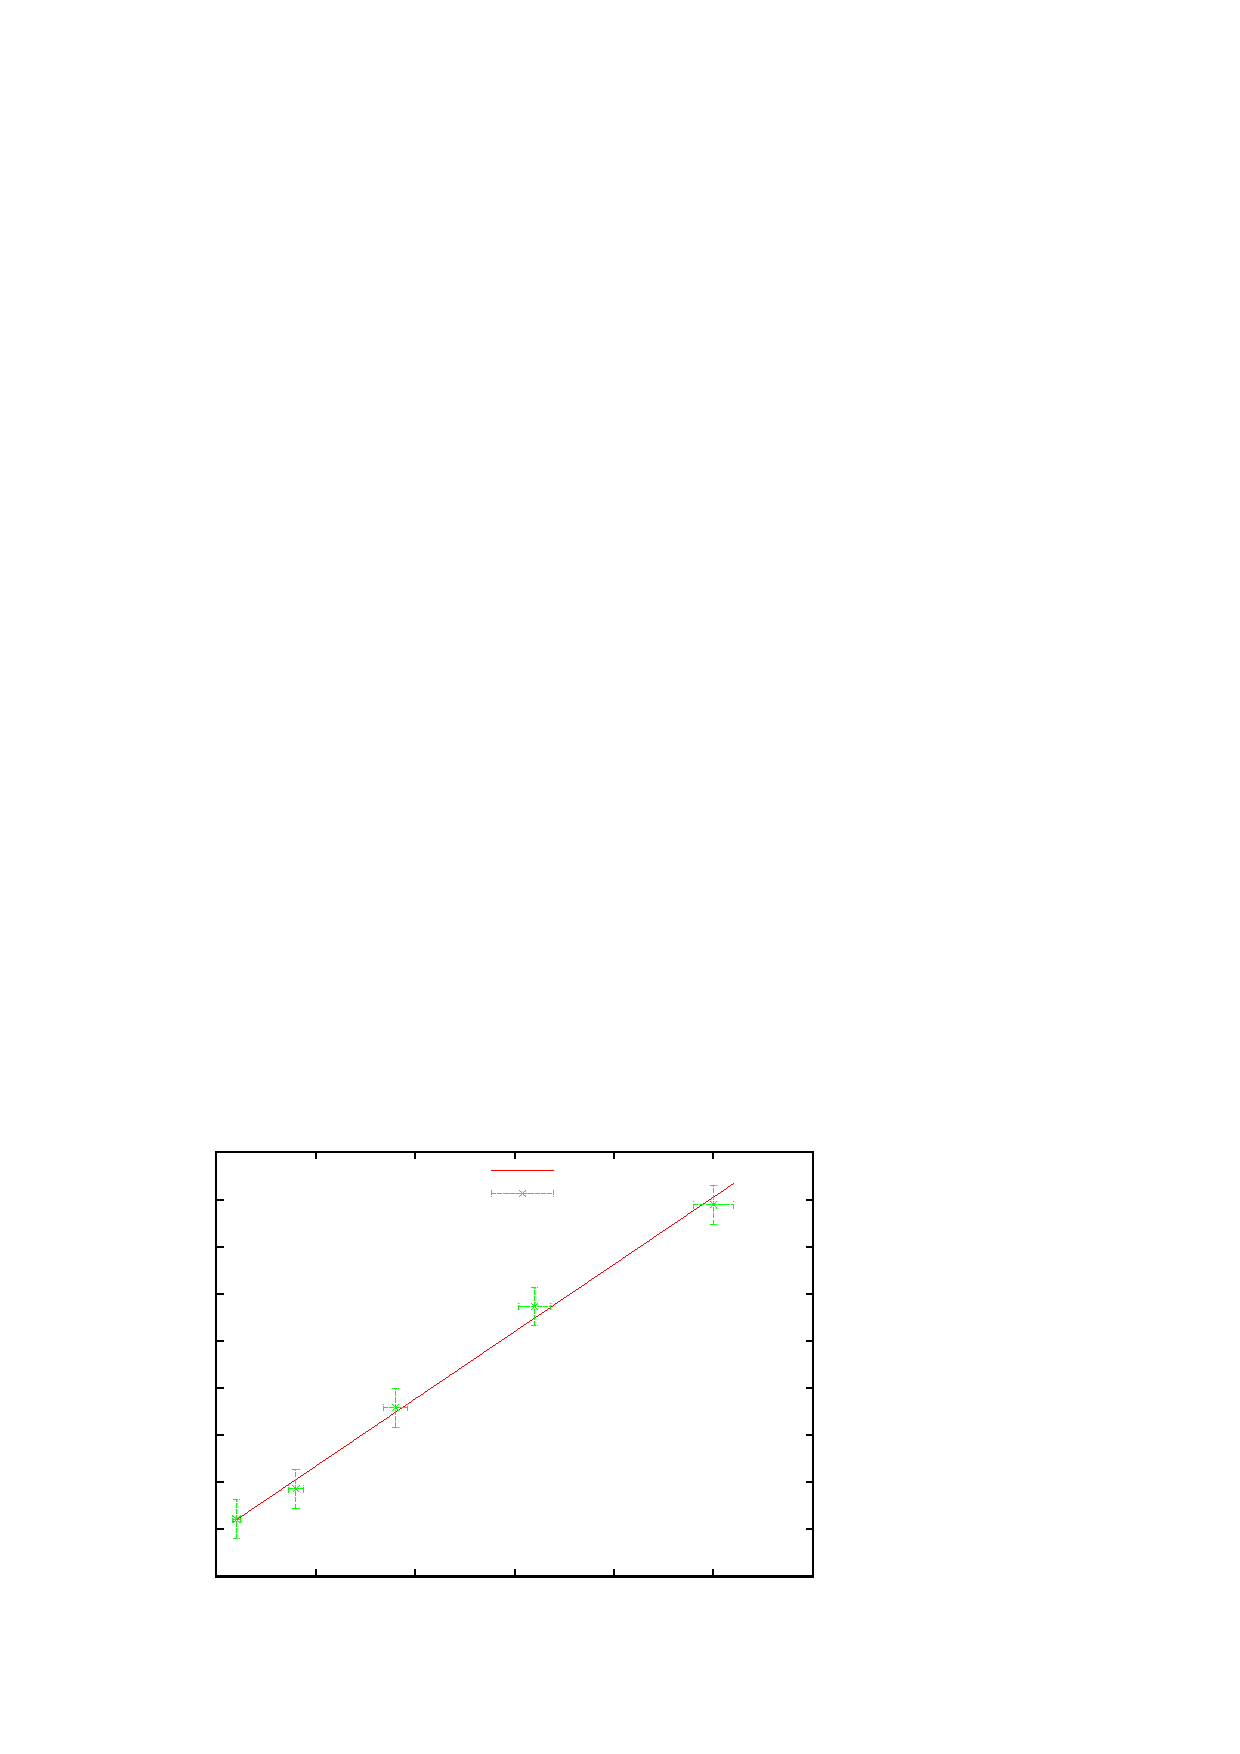
\includegraphics{kondwarm}}%
    \gplfronttext
  \end{picture}%
\endgroup

\caption{Energie des Kondensators aufgetragen gegen die Änderung im Druck}
\label{fig:druckwarm}
\end{figure}
Aus der durchgeführten linearen Regression ergibt sich eine Steigung von $m=(108\pm5)\frac{\text{J}}{\text{Pa}}$
bei einem reduziertem $\chi^2$ von 1.1.
Um die Freiheitsgrade des Gases zu bestimmen, nehmen wir uns die Formel \eqref{eq:fhalbe}
aus der Theorie.
Hier wird angenommen, dass $\Delta V=0$ ist, da das Volumen konstant bleibt.
Daraus ergibt sich diese Formel für die Freiheitsgrade f, wenn man $\frac{\Delta Q}{\Delta p}=\frac1m$ setzt, wo bei m die Steigung der Regressionsgeraden ist.
\begin{align}
	f= \frac{2\cdot \Delta Q}{V\cdot \Delta p}=\frac{2}{V\cdot m}
\end{align}
Das hierbei verwendete Volumen berechneten wir aus den aufgenommenen Maßen des Zylinders, welche $r=(0.044\pm 0.002)$m für den Radius und $h=(0.400\pm 0.005)$m für die Höhe betrugen.
Der Fehler ergibt sich aus der Gauß'sche Fehlerfortpflanzung.
\begin{align}
	\sigma_f=\sqrt{\sigma_V^2\left(\frac{-2}{V^2\cdot m}\right)^2+\sigma_m^2\left(\frac{-2}{V\cdot m^2}\right)^2}
\end{align}
Hierraus ergeben sich die unten aufgeführten Freiheitsgrade.
$$\shadowbox{$f=(8\pm 1)$}$$
Dies ergibt eine Abweichung von fast $40\%$ zum Literaturwert $f=5$, da Luft zu $99\%$ aus Stickstoff (N$_2$) und Sauerstoff (O$_2$) besteht, welche jeweils 5 Freiheitsgrade haben.

\subsubsection{Spezifische Wärme $c_v$}
Aus den oben berechneten Freiheitsgraden der Luft kann man jetzt mit der gleichen Formel \eqref{eq:fhalbe}
, wie oben die Spezifische Wärme $c_v$ der Luft berechnen.
Es ergibt sich durch umstellen der Formel, die hier aufgeführte Formel.
\begin{align}
	c_v=\frac{f\cdot R}{2}
\end{align}
Durch die Gauß'sche Fehlerfortpflanzung ergibt sich die Gleichung für den Fehler (unter der Voraussetzung, dass nur f fehlerbehaftet ist).
\begin{align}
	\sigma_{c_v}= \sqrt{\sigma_f^2\left(\frac{R}{2}\right)^2}
\end{align}
Es ergibt sich ein Wert für die spezifische Wärme von Luft.
$$\shadowbox{$c_v=(33\pm 5)\si{\joule/\mol\kelvin}$}$$
Dies ist eine Abweichung von $40\%$
zum Literaturwert von $c_v=20.7\si{\joule/\mol\kelvin}$ \cite[S. 260]{gerthsen}.

\section{Diskussion}
\label{sec:diskussion}
\subsection{Gasthermometer}
Unser Wert für die Nullpunktstemperatur hat eine Abweichung von 8\% zum Literaturwert.
Diese Abweichung ist ziemlich gering, dennoch liegt der Literaturwert nicht im Fehlerintervall.
Als mögliche Fehlerquelle kann man aufführen, dass wir das Manometer nicht ganz richtig bedient haben.
Es ist wahrscheinlich, dass wir keinen vollständigen Druckausgleich des Gefäßes mit der Außenluft duchgeführt haben.
Wir haben somit nicht den Außendruck bei einer Temperatur von 0\si{\celsius}.
Dies sorgt dafür, dass die sich ergebene Grade einen zu höheren y-Achsenabschnitt hat, als sie sollte und damit die Nullpunktstemperatur niedrieger ist, als die des Literaturwertes.
Dies können etwa 8hPa gewesen sein, die somit unser Ergebnis verfälscht haben.

\subsection{Spezifische Wärme der Luft}
Unsere Messung der Freiheitsgrade der Luft weicht um $40\%$ vom Literaturwert ab.
Allerdings ist unser Fehlerintervall auch relativ groß, wenn es auch den theoretischen Wert nicht mit einschließt.
Im Vergleich zu anderen Arbeiten ist unsere Geradensteigung zu klein (andere haben Werte von ca. $m=130$).
Vermutlich haben wir durch die hohe Geschwindigkeit, mit der abgelesen werden musste, viele fehlerbehaftete Werte notiert.
Um dies in zukünftigen Arbeiten zu beheben, wäre es eine Möglichkeit, eine Kamera auf die Skala zu richten und die Messungen aufzunehmen.

\section{Messwerte}
\subsection{Gasthermometer}
\begin{table}[!htb]
	\centering	
	\begin{tabular}{|c|c||c|c|}
	\hline
	Temperatur [$\si{\celsius}$]  & Überdruck (x2=kPa)&
	Temperatur [$\si{\celsius}$]  & Überdruck (x2=kPa)\\
	$\sigma=0.5\si{\celsius}$ & $\sigma=0.03~$kPa &
	$\sigma=0.5\si{\celsius}$ & $\sigma=0.03~$kPa \\
	\hline
	0	&	-0.04	&	47	&	8.29	\\
	1	&	0.2	&	50	&	8.75	\\
	2	&	0.35	&	52	&	9.13	\\
	5	&	0.95	&	55	&	9.66	\\
	7	&	1.22	&	57	&	10.01	\\
	10	&	1.88	&	60	&	10.49	\\
	12	&	2.12	&	65	&	11.38	\\
	15	&	2.81	&	68	&	11.8	\\
	17	&	3.14	&	70	&	12.22	\\
	20	&	3.67	&	73	&	12.68	\\
	23	&	4.18	&	75	&	12.95	\\
	25	&	4.47	&	77	&	13.29	\\
	27	&	4.87	&	80	&	13.89	\\
	30	&	5.34	&	85	&	14.7	\\
	32	&	5.7	&	88	&	15.22	\\
	35	&	6.15	&	90	&	15.57	\\
	38	&	6.6	&	92	&	16.05	\\
	40	&	6.99	&	95	&	16.41	\\
	42	&	7.44	&	98	&	17.22	\\
	45	&	7.96	&		&		\\
	\hline
	\end{tabular}
	\caption{Erwärmen bei einem Umgebungsdruck von $1014.0\pm 0.1~\si{\hecto\pascal}$}
\end{table}

\begin{table}[!htb]
	\centering	
	\begin{tabular}{|c|c||c|c|}
	\hline
	Temperatur [$\si{\celsius}$]  & Überdruck (x2=kPa)&
	Temperatur [$\si{\celsius}$]  & Überdruck (x2=kPa)\\
	$\sigma=0.5\si{\celsius}$ & $\sigma=0.03~$kPa &
	$\sigma=0.5\si{\celsius}$ & $\sigma=0.03~$kPa \\
	\hline
	92	&	15.93	&	45	&	7.97	\\
	90	&	15.44	&	40	&	7.15	\\
	88	&	15.1	&	35	&	6.29	\\
	85	&	14.51	&	30	&	5.45	\\
	80	&	13.8	&	23	&	4.18	\\
	75	&	12.93	&	20	&	3.72	\\
	70	&	12.14	&	15	&	2.7	\\
	65	&	11.31	&	10	&	1.55	\\
	60	&	10.52	&	5	&	0.81	\\
	55	&	9.65	&	0	&	-0.03	\\
	50	&	8.81	&		&		\\
	\hline
	\end{tabular}
	\caption{Abkühlen  bei einem Umgebungsdruck von $1014.0\pm 0.1~\si{\hecto\pascal}$}
\end{table}

\subsection{Spezifische Wärme der Luft}
Die verwendeten Kondensatoren haben eine Kapazität von $10~\si{\micro\farad}$ und sind parallel geschaltet.


\begin{table}[!htb]
	\centering
	\begin{tabular}{|c|c|}
	\hline
	$U$ [V] & $h$ [mm]\\
	$\sigma_U=10~$V & $\sigma_h=0.1~$mm\\
	\hline
	100	&	2	\\
	150	&	1	\\
	200	&	5	\\
	250	&	6	\\
	300	&	10	\\
	350	&	12	\\
	400	&	18	\\
	450	&	22	\\
	500	&	26	\\
	500	&	25	\\	
	\hline
	\end{tabular}
	\caption{Steighöhe in Abhängigkeit der am Kondensator angelegten Spannung}
\end{table}

\begin{thebibliography}{100}

\bibitem{gerthsen}
	\textsc{Dieter Meschede} (2010): \emph{Gerthsen Physik}, 24. Auflage, Springer Heidelberg
Dordrecht London New York

\bibitem{lp} 
	\emph{Lehrportal der Universität Göttingen, Spezifische Wärme der Luft und Gasthermometer},
  http://lp.uni-goettingen.de/get/text/3643, abgerufen 23.07.14 11:13 Uhr

\end{thebibliography}


\end{document}
